\documentclass{article}
\usepackage[english]{babel}
\usepackage[utf8]{inputenc}\usepackage{fancyhdr}
\usepackage[square]{natbib}
\usepackage{multibib}
\newcites{main}{Primary References}
\bibliographystyle{apalike}
\bibliographystylemain{apalike}
\newcites{code}{Code References}
\bibliographystylecode{apalike}
\newcites{soft}{Software References}
\bibliographystylesoft{apalike}
\usepackage{graphicx}
\graphicspath{ {./Images/} }
\usepackage{geometry}
\geometry{a4paper,left=30mm,top=30mm}
\usepackage{hyperref}
\usepackage{float}

%Titlepage
\thispagestyle{fancy}
\fancyhf{}
\setlength{\headheight}{22.54448pt}
\rhead{University of Sussex - Informatics\\
Computer Science with Artificial Intelligence}
\lhead{Jacob Brown}
\rfoot{
Submission Year - 2022\\
Candidate Number - 198732\\
Project Supervisor - Simon Bowes\\
}

\begin{document}
\paragraph*{
\\
}
\part*{
\begin{center}
{ \Huge "Lizardbot"}
\\[1\baselineskip]
{\Large A reptile-inspired model of robots optimised to navigate rough terrain}
\end{center}
}
\paragraph*{Abstract\\}
Insert abstract here
\vspace*{\fill}
\newpage
\pagestyle{fancy}
\fancyhf{}
\rhead{PAGE \thepage}
\lhead{LIZARDBOT - \leftmark}

\tableofcontents

%Report
\newpage
\section{Introduction}
Add in the intro pretty much directly from the interim report here

\newpage
\section{Project Aims}
Why is the robot being modelled instead of physically built?\\
Why did I choose to use Unity?\\
\subsection{Primary Objectives}
\subsubsection{Robot Design}
Get from interim report - explain overall design and why those decisions were made e.g. simplistic design
\subsubsection{Robot Movement}
Basic overview of why each component will move the way it does. Tie each point back to how they are founded (or not founded) in natural algorithms.\\ 
Include jumping here\\
\subsubsection{Terrain Generation}
The terrain will be static - why?\\
Why will I have three separate terrains? - Octopus\\
What is the importance of having a smooth terrain?\\
\subsubsection{AI}
How will the AI work? Genetic algorithm outline\\
Dynamic systems theory\\
Damage minimisation\\
How do I want the AI to manipulate the relationship between the body and movement?\\
Why do I want there to be a relationship between the two? - article Simon sent\\
How am I going to test the relationship?\\
How will the robot be measured?\\

\subsection{Extension Objectives}
\subsubsection{Vision}
How would a rudimentary visual system reduce damage to the robot?\\
How would this move the AI from a reactive to proactive mechanism?\\
\subsubsection{Terrain Friction}
How do snakes work with different frictions?\\
\subsubsection{UI}
How could a UI help lower the threshold to the project and make it easier to 'work with' the AI?\\
\subsubsection{Flexible Tail}
What are the advantages of having a flexible tail?\\


\newpage
\section{Project Relevance}
\subsection{Salamandra Robotica II}
Insert from interim report
\subsection{Agama Robot}
Insert from interim report
\subsection{tbc}
Find a team that have modelled a robot vs building one

\newpage
\section{Requirements Analysis}
Insert from interim report - needs some work\\
Add section on the constraints of this project

\newpage
\section{Professional and Ethical Considerations}
Insert from interim report with more reference to code of conduct

\newpage
\section{Implementation}
\subsection{Terrain}
Three terrains were generated using Procedural Toolkit \citepsoft{proceduralToolkit} to test the performance of the robot across various environments: rough, uneven, and smooth. These categories were inspired by the those used by the Octopus robot \citepmain{octopusRobot}.\\
\begin{figure}[H]
\centering
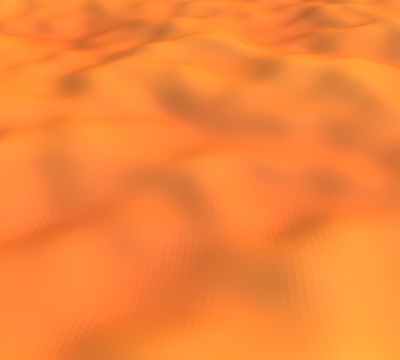
\includegraphics[scale=0.3]{smoothTerrain}
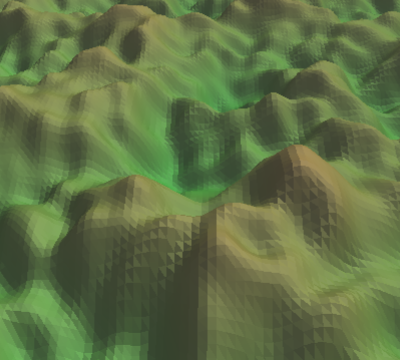
\includegraphics[scale=0.3]{unevenTerrain}
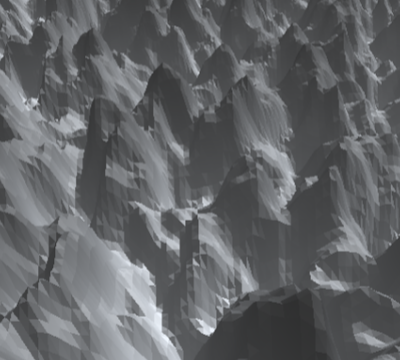
\includegraphics[scale=0.3]{roughTerrain}
\caption{Examples of the three terrain types. From left to right: Smooth, Uneven, Rough.}
\end{figure}
At one point the height of the terrain was proportional to the number of sections of the robot, a similar method to that of the Octopus robot. However, as the terrain is a control variable the heights were switched to a static value: $Smooth=8, Uneven=16, Rough=24$.\\
Overall, the rougher the terrain, the higher and more closed in it is. Most of the development of the robot was conducted on the smooth and uneven terrains, as the rough terrain aims to provide a more extreme environment with which to test the efficacy of the AI.\\
The smooth terrain is deliberately featureless to test the behaviour of the robot in a simple environment. Herbert Simon provided an elegant example of the importance of this consideration: an ant is observed making its way back to its nest across a beach.\\
Its route is ‘a sequence of irregular, angular segments’ that suggests some level of complexity in the ant's behaviour. However, the beach for the ant is a much harsher environment than it is for a human. It is more likely that ‘its complexity is really a complexity in the surface of the beach, not a complexity in the ant.’ \citepmain{antsBeach} Thus, the situatedness of the robot could culminate in behaviours that are not of its own making and are instead caused by its relationship with the terrain. The smooth terrain should reduce the role of the environment and allow for emergent behaviours to be prescribed to the robot itself. It is worth noting that the robot is still being tested on three terrains with some common properties (e.g. gravity) and these factors may introduce bias in the AI. This is a reasonable situation as long as applications of the Lizardbot are further modelled on encounterable terrains to allow the AI to adapt the robot accordingly. For proof of concept the sample set of terrains is sufficient.

\subsection{Robot}
\subsubsection{Body}
To create a snakelike body, each body module is attached to the previous module by a configurable joint \citepcode{configJoints} and has two methods of movement: driving and rotation. The physical design of the robot creates a fluid motion before any complex movement is applied. With the joint structure, the movement of one section is translated to those behind it - similar to dragging a piece of string along the ground. This is shown in figure x: the head rotates and, after a delay, creates the same angle in the sections behind it.\\
The former applies a forward force as determined by the drive velocity parameter whilst the latter applies a velocity to each module using the following equation:
\begin{center}
\begin{Large}
$\overrightarrow{v_{i}} = \overrightarrow{v_{i-1}} + \frac{m}{2}\overrightarrow{w} $
\end{Large}
\end{center}
For rotating sections $i = 0, ..., m$, where $m \leq n$, the value of $w$ will be calculated using $S$ or $C$ as specified.\\
\begin{center}
\begin{Large}
$S: \overrightarrow{w} = sin\overrightarrow{\theta_{i-1}} + sin\overrightarrow{\theta_{i}}$
\\[1\baselineskip]
$C: \overrightarrow{w} = cos\overrightarrow{\theta_{i-1}} + cos\overrightarrow{\theta_{i}}$\\
\end{Large}
\end{center}
This central pattern generator (CPG) approach allows each module to react to the velocity and angle of the previous section. The equation for the CPG originated in Tony Dear’s multi-link snake robot: a robot with a similar modular design with passive joints connecting the modules. \citepmain{cpgRobot} Lizardbot utilises the same math to calculate the velocity with one distinction: Dear’s robot split the velocity vector into its axes, using cos for the x axis and sin for the y. Lizardbot instead calculates the vector as a whole and alternates the rotating sections between sin and cos to produce the serpentine motion. For robots with serpentine motion disabled, $S$ and $C$ will be assigned randomly to the rotating modules.\\

\begin{figure}[H]
\begin{minipage}[b]{.4\textwidth}
\centering
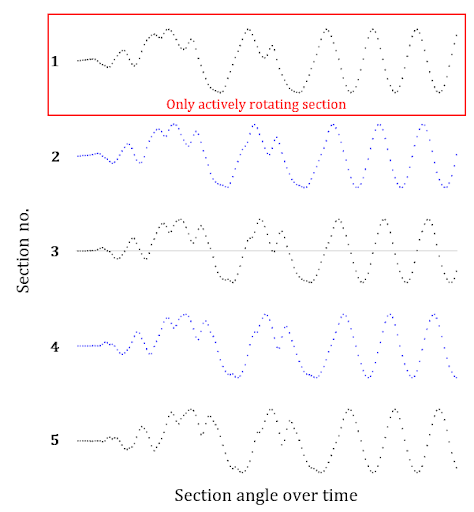
\includegraphics[width=1\textwidth]{cpgMirroring}
\caption{Demonstration of body motion with a single rotating section at the head of the body.}
\end{minipage}
\hfill
\begin{minipage}[b]{.5\textwidth}
\centering
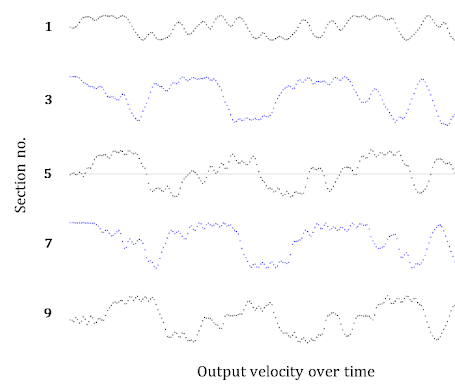
\includegraphics[width=1\textwidth]{cpgSerpentine}
\caption{The output velocities generated by each body module with serpentine motion enabled. Modules using $S$ are shown in black, $C$ in blue.}
\end{minipage}
\end{figure}

As each section ‘reacts’ to the previous one whilst using the opposing equation, the velocity applied is almost an inversion of its predecessor. Moving back through the body there appears to be more fluctuation in the values as more noise is introduced through each application of the equation. The advantage of using this recursive approach is the incredibly organic behaviour that it produces. The first prototypes of the project used hardcoded timings and velocities to try and mimic a serpentine motion and the rigidity of the code was evident in the behaviour. With the above equation applied, the motion of the body appears completely natural. As the Lizardbot slithers through troughs in the terrain or wriggles whilst stuck on a ridge, it is easy to forget that it has no awareness of its surroundings. It is simply reacting to the body that came before it.


\subsubsection{Tail}
The use of a tail has the potential to counterbalance the body and provide stability as the lizardbot moves. The Agama robot used the angular momentum of the body to calculate how to calibrate the tail vertically as the robot jumped. Lizardbot implemented a similar approach in three dimensions by calculating the total momentum of the robot around its centre of gravity (COG) at each frame, and adjusting the velocity of the tail accordingly.\\ 
\begin{figure}[H]
\centering
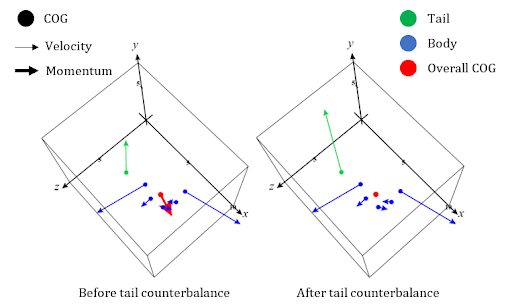
\includegraphics[scale=0.6]{tailMomentum}
\caption{A representation of the tail being adjusted to conserve the angular momentum of a robot. Diagram created using CalcPlot3D \citep{diagrams}}
\end{figure}

For all body parts $i = 0, ..., n$, the radius of the path of motion is the distance from the individual COG $x$ to the COG of the overall robot.
\begin{center}
\begin{Large}
$r = |x_{i} - \frac{1}{n}\sum_{i}^{n}m_{i}x_{i}|$
\end{Large}
\end{center}
The total angular momentum $L$ of the robot is calculated using the above values of $r$, the mass $m$ and the velocity $v$ of each body part. \citepcode{angularMomentum}
\begin{center}
\begin{Large}
$L = \sum^{n}_{i} r_{i}m_{i}v_{i}$
\end{Large}
\end{center}
To conserve momentum, the velocity of the tail is calculated by inverting $L$ and dividing it by the tail's mass and distance from the overall COG.
\begin{center}
\begin{Large}
$v_{t} = - \frac{L}{r_{t}m_{t}}$\\
\end{Large}
\end{center}

Another simplified approach was considered whereby the overall velocity of the robot was counterbalanced instead, however this was found to create sharp changes in the velocity of the tail that could cause it to fling the entire body into the air. Whilst this showed promising behaviour for the basis of a jumping motion, it was counter-productive for a feature whose goal was to stabilise the robot. Additionally, by calculating the magnitude around the COG, any difference in mass between components is taken into consideration. Thus, the tail is able to counterbalance any body structure (assuming that the motion of the tail is not physically blocked by the position of a body part).\\

The design of the tail assumes that nature has already selected for the optimal location by placing the tail at the back of a creature. This assumption seems intuitive. Most animals, including lizards, are symmetrical and the location of the tail maintains this property, alongside keeping the motion of the tail in the same plane as the rest of the body. For Lizardbot, this assumption could be removed in the future. Since symmetry is not a required property for non-uniform bodies, the tail could be placed anywhere that has equal mass either side of the tail - or placed randomly to see what effect this has on the robot. Who am I to say that a tail cannot be located on the head?

\subsubsection{Legs}
Legs were added to Lizardbot in an attempt to match the gait of a lizard.
As inspired by the design of the Salamandra Robotica \citepmain{salamandra}, each leg is designed to rotate in a circle in order to push the body forward. The physical design of the leg matches the elliptical shape of the tail and uses the same configuration of customisable mass and length. 
Currently, there are only two attachment points for a leg on each body module: one each side, perpendicular to the body joints. For a uniform body, the legs are placed symmetrically along the body and given equal length and mass; they are constructed randomly for non-uniform bodies. \\

The leg rotates around an axis perpendicular to the body section it is attached to, as shown in figure x. The size of the circle it follows is determined by the angle it is offset by when attached to the body ($\alpha$). \\

\begin{figure}[H]
\centering
$\vcenter{\hbox{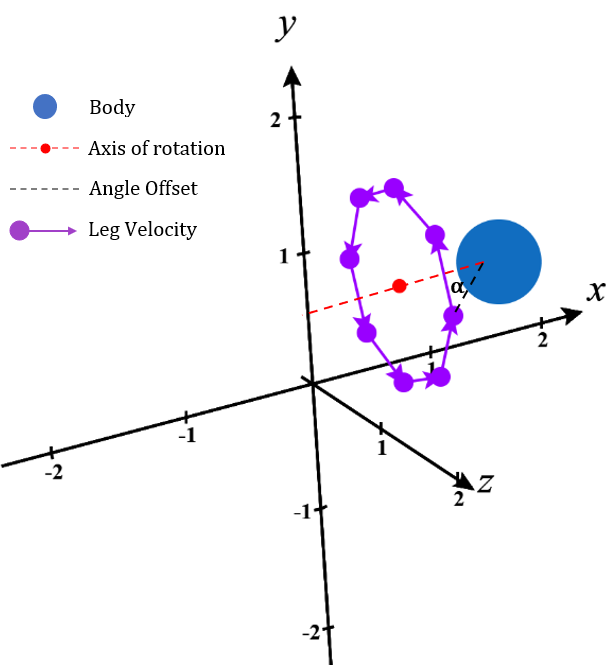
\includegraphics[width=0.5\textwidth]{legCircleDiagram}}}$
$\vcenter{\hbox{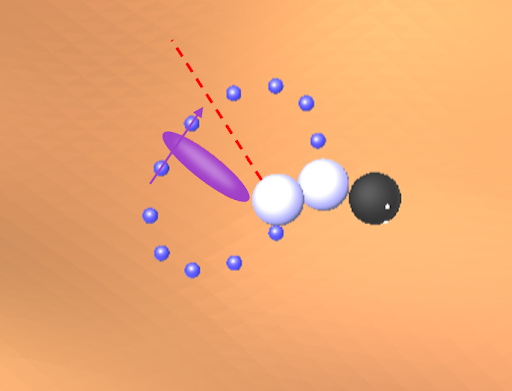
\includegraphics[width=0.4\textwidth]{legCircleExample}}}$
\caption{\\Left: An illustration of the rotation of a leg around an axis of rotation. Only one attachment point is shown - another would be available on the other side of the body along the $x$ axis.\\
Right: A leg following its path of motion.}
\end{figure}



The rotation of the leg follows a series of conceptual points spaced $30^\circ$ apart around the point $D$ (shown by the red point along the axis of rotation in figure x). These points are generated using the following equation:
\begin{center}
\begin{Large}
$P = D + Vcos\theta + Ucos\theta$\\
\end{Large}
\end{center}
Where $V$ and $U$ are two vectors perpendicular to each other in a plane through $D$ and the target circle, and $0\leq\theta<360$. \citepcode{circlePoints}
 
To calculate the desired velocity of the leg, the point $P_i$ closest to the current position of the leg is found. From this, the new velocity can be calculated using the vector to the next point on the circle.   
\begin{center}
\begin{Large}
$v_{i} = g(P_{i + 1} - P_{i})$
\end{Large}
\end{center}
If the relevant gene is active, the gait multiplier $g$ increases the velocity when the body is turning away from the leg, decreasing it if the body is turning toward the leg.\\

The performance of the legs is analysed in section x, though it is presumed that with more work the performance could be drastically improved: currently it resembles a lot of twitching. It is possible that an alternative joint mechanism would allow for Lizardbot to stand on its legs and appear more natural. It would also be interesting to explore how the location of the legs impacts the robot as a whole. Currently the attachment points are based on lizards (indeed, most animals) and the years of evolution that have led to their structure. However, the offer of more variety in the design of the robot may offer alternative solutions to navigate the terrain. 


\subsection{Artifical Intelligence}
A population of Lizardbots can use a genetic algorithm to "evolve" over a series of generations. A genetic algorithm is a form of artificial intelligence that more closely models the characteristics of natural selection. An agent’s parameters are broken down into ‘genes’ that can be manipulated by recombination and/or mutation. The aim of this genetic algorithm (GA) is to improve the performance of the robots over time. The GA is performed when a robot is declared to be stuck by the trapped algorithm. 

\subsubsection{Performance}
The metric used to measure the performance of a robot can heavily influence the outcome of the genetic algorithm. As the desired outcome is a robot capable of navigating the terrain, the base measurement used is the furthest distance (by magnitude) that it has travelled in a given generation from its spawn point within the terrain. 
\\[1\baselineskip]
Two additional parameters are used to add context to this base measurement. 

The first penalises robots that cause large collisions through a body part. Every time a body part encounters a collision it triggers a method that will measure the force that the body part has experienced. Unity's build-in physics system returns the impulse $I$ of a collision. Using this, the force can be found by dividing the impulse by time: {\Large $f = \frac{I}{t}$}. \citepcode{collisionForce}
If the force is found to be above a threshold then the robot will be penalised by deducting 10\% from the performance. \\
This ensures that the robot is not evolving toward a behaviour that carries it across the terrain efficiently but could be damaging to its structure in the physical world. An example of this is an iteration whereby the robots were observed ‘flicking’ their tails rapidly downward, causing the robot to be thrown into the air and across the terrain. Whilst this was effective at getting them to the edge of the terrain within seconds, this approach would shatter most robots upon collision with the terrain. This threshold can be tailored to the needs of the robot, such that robots with shielding or soft-bodies robots can be given a higher threshold to allow more risky behaviour.

The second rewards robots that move quickly. The current performance is multiplied by the average speed (distance / time) of the robot since its spawn. 
\\[1\baselineskip] 
To provide an example of the performance metric, say Robot3 V8 has travelled from (0, 0, 0) to (10, 4, -13) in 21 seconds, and has had two above-threshold collisions. The base performance would be 16.88. Multiplied by its speed, this becomes 13.57. With a 10\% deduction for each collision, the final performance is 10.99. \\
A flaw in this metric is that it does not differentiate between the routes that robots take. If one robot moved quickly but erratically, it may be rewarded equally to one that moved slowly and directly. However, this metric appears to provide a suitable balance between rewarding robots that travel the furthest, further rewarding those that move efficiently, and reducing behaviours that would damage a physical robot. \\

When referring to the performance of a population, the mean performance of the highest performing 25\% is being measured. When a robot is mutated and respawned its performance returns to zero, hence it was found that analysing the entire population added too much noise to the results. 

\subsubsection{Trapped Algorithm}
It is important for the AI to know when the robot is stuck to trigger the termination of the current generation. At this point the AI can mutate the robot before respawning it. This trapped behaviour can take many forms, from bouncing against the same point in the terrain, circling itself, or looping between the same location(s).\\

Initially, the maximum - minimum of the baseline performance metric (magnitude of the distance from the origin) over the last $t$ seconds was used. This approach was heavily flawed as it reduced the data set to a single dimension. \\
Instead, the entire data set over the last $t$ seconds was analysed. The robot was declared stuck when the variance of the robot’s 3D coordinates over $t$ seconds converged to 0. This approach correctly identified the robot as stuck but had one major flaw: travelling in a straight line outputs a variance of 0. This behaviour is highly efficient and, whilst it is not something that the AI will train for, is a behaviour that the AI should absolutely not be training against. These false positives prompted a third approach. \\
The algorithm finds the minimum and maximum values for each axis to draw a conceptual cube around the points the robot has visited in the last $t$ seconds. These cubes depict the  worldspace the robot has recently explored. The variance of the data set is calculated for the volume of the cube rather than the coordinates themselves. If the variance of the volumes of the cubes rounds to zero then the robot is considered to be trapped. \\
\begin{figure}[H]
\centering
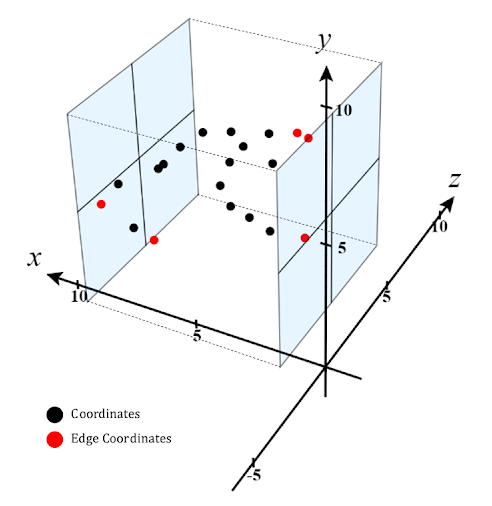
\includegraphics[scale=0.7]{trappedAlgorithm}
\caption{A representation of the cube constructed around the last 20 locations a robot has visited (captured twice a second).}
\end{figure}

Finally, the sensitivitiy of the algorithm needed to be determined by adjusting the value of $t$. The results showed that too low a value of $t$ produced false positives due to it not allowing the robot enough time to turn around. In contrast, if $t$ was too high it took longer for the algorithm to identify when the robot was stuck. This would waste time continuing for an extra few seconds each generation, or could potentially miss instances when the robot became trapped but was able to free itself. A sensitivity of $t=20$ appeared to provide a balanced value across all three terrains.

\begin{figure}[H]
\centering
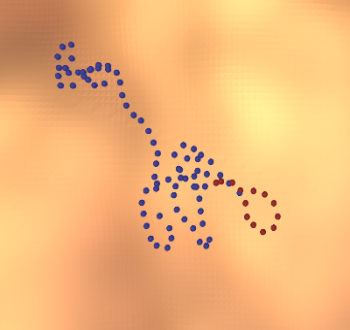
\includegraphics[width=0.2\textwidth]{trappedSmooth}
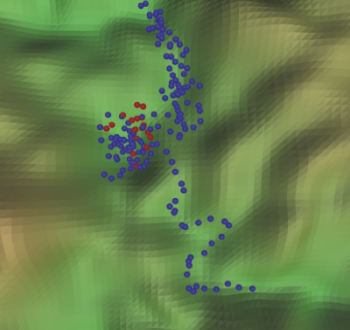
\includegraphics[width=0.2\textwidth]{trappedUneven}
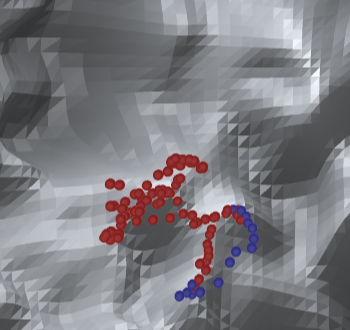
\includegraphics[width=0.2\textwidth]{trappedRough}
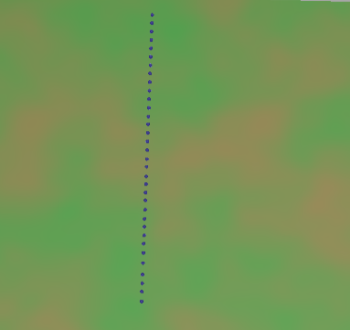
\includegraphics[width=0.2\textwidth]{trappedFlat}
\caption{A demonstration of the trapped algorithm using the same robot and $t=20$ on each terrain.\\
Each blue point represents the location of the robot being captured. Red indicates that the robot is trapped (and would normally have been disabled and passed to the genetic algorithm).\\ 
From left to right: Smooth, Uneven, Rough, Flat. The latter used a robot with rotation disabled to ensure that a robot travelling in a straight line would not be flagged.}
\end{figure}
The red points in figure x align with behaviours that can reasonably be classed as ‘trapped’, however it is important to note that this algorithm was implemented with some bias toward certain behaviours (e.g. looping). For this project, the identification of a trapped robot appears sufficient and is expected to produce an AI that will train away from continually exploring the same area for too long. The algorithm has other potential applications in finding looping patterns in any problem that can be assigned a world space. For example, a neural network could be analysed with this algorithm to determine when it is ‘stuck’ whilst performing a task, or a search algorithm could implement it to avoid excessively exploring within a section of the graph. 


\subsubsection{Genes}
The manipulatable characteristics of a robot are distinguished by a \textit{Gene} class. Each variable is instantiated with a default, minimum, and maximum value. Additionally, they are given a type (established in the enum class \textit{Variable} whereby negative enum values are physical properties and positive are movement) to ensure that the recombination covered in section x is combining the same genes with each other. \\
This class handles any erroneous situations that arise and allows boolean values to be stored as a float. If the \textit{Get} method of a boolean \textit{Gene} is called, then true will be returned for values greater than 0.5. This allows boolean genes to be mutated slowly (e.g. from 0.35 to 0.6) without having to make a single toggle from one value to the other. \\
When a gene is mutated, if the new value lies outside the valid range then it is 'bounced' (e.g. $max=0.5, v\rightarrow0.6 \Rightarrow v=0.4$). If a value outside the max/min values is passed directly then the max/min value would be assigned instead.

\subsubsection{Population}
To avoid interaction between robots, the body parts of a robot should be capable of colliding between themselves and the terrain but should ignore those of other robots. In Unity, this can be achieved by placing all robot objects into a layer. You can then change the Physics system to ignore collisions between different robot layers.\\ 
Unity’s layers have a limit of 25 available layers. At first, a script was added to every robot scanning around it for other robots in the same layer. Upon detection, the current robot would be moved to another layer that no robots in the vicinity were using. Given that every robot spawned in the same location this script absolutely throttled the performance of the program. With a population of 50 the frame rate would drop from ~200fps to ~20fps. This is not an acceptable impact so an alternative approach was considered. Multiple terrains are generated and 25 robots placed into each. This has the added benefit of being able to generate a population of robots being tested on all three terrain types simultaneously. 


\subsubsection{Genetic Algorithm}
When a gene is mutated its value, v, is adjusted as follows:
\begin{Large}
$G_{i} = R^{[0, 1]} < m \longrightarrow 
(max(G_{i}) - min(G_{i})) R^{[0.01, 0.1]}  G_{i}$\\\\
$G(1)_{i} = R^{[0, 1]} < r \longrightarrow$ 
\begin{LARGE}
$^{R^{[0, 1]} < 0.5\longrightarrow G(1)_{i}} 
_{R^{[0, 1]} \geq 0.5 \longrightarrow G(2)_{i}}$\\\\
\end{LARGE}

\end{Large}
where R denotes a randomly generated number. G(1) refers to the input robot, whilst G(2) is the selected robot. For \textit{Triad} recombination G(2) is randomly chosen from either of the two selected robots, with equal probability.
\subsection{Dynamic Movement}
Insert from DST log

\subsection{UI}


\newpage
\section{Results}
How does mutating the body / movement independently work?\\
How does the addition of the tail help?\\
How does initiating the body with a serpentine motion established affect the outcome?\\
What happens when the body is set as static?\\
What is the outcome when the legs are out of sync from the body?\\
Starting with defaults, what parameters does the AI mutate to? What is the corresponding behaviour for this?\\
Does the AI converge on the same parameters when started with different defaults?\\



\newpage
\section{Conclusion}

\newpage

\section{References}
\nocitesoft{*}
\nocitecode{*}

\bibliographymain{References/References}
\bibliographysoft{References/SoftReferences}
\bibliographycode{References/CodeReferences}
\newpage
\section{Appendices}
\subsection{Code of Conduct}





\end{document}